Many classical computer vision applications such as stereo, optical flow, semantic
segmentation and visual grouping can be naturally formulated as image labeling tasks.

Arguably the most popular way to approach such labeling problems is via graphical
models, such as Markov random fields (MRFs) and conditional random fields (CRFs).
MRFs and CRFs provide a principled way of integrating local evidence and
modeling spacial dependencies, which are strong in most image-based tasks.

While in earlier approaches, model parameters were set by hand or using
cross-validation, more recently parameters are often learned using a max-margin
approach.

Most models employ linear energy functions of unary and pairwise interactions,
trained using structural support vector machines (SSVMs). While linear energy
functions lead to learning problems that are convex in the parameters, complex
constraints complicate their optimization. 

In recent years there has been a wealth of research in methods for learning structured prediction,
as well as in their application in areas such as natural language processing and computer vision.
Unfortunately only few implementations are publicly available---many applications are based on
the non-free implementation of~\citet{joachims2009cutting}.

In this chapter, we will first introduce the concepts and algorithms used in structured prediction,
in particular in maximum margin methods. We will then accompany this by a description of our
open source implementation of these algorithms, \pystruct.

\pystruct aims at providing a high-quality implementation with an easy-to-use
interface, in the high-level Python language.  This allows practitioners to
efficiently test a range of models, as well as allowing researchers to compare
to baseline methods much more easily than this is possible with current
implementations.  \pystruct is BSD-licensed, allowing modification and
redistribution of the code, as well as use in commercial applications.  By
embracing paradigms established in the scientific Python community and reusing
the interface of the widely-used {\sc scikit-learn}
library~\citep{pedregosa2011scikit}, \pystruct can be used in existing
projects, replacing standard classifiers.  The online documentation and
examples help new users understand the somewhat abstract ideas behind
structured prediction.

%The organization of this chapter is as follows. Section~\ref{sec:api} revisits
%the basic concepts of structured learning algorithms, and how these map to the
%\pystruct interface. Section~\ref{sec:examples} exemplifies the use of \pystruct
%on some standard structured prediction benchmarks and showcasts how \pystruct
%can interact with existing libraries, foremost scikit-learn and scikit-image.
%Section~\ref{sec:benchmarks} finally compares \pystruct with SVM$^\text{struct}$,
%arguably the most widely used implementation of structural SVMs, and
%SVM$^\text{python}$, a Python interface or the same.

\section{Basic Concepts in Structured Prediction}

Structured prediction can be defined as making a prediction $f(x)$ by maximizing a
compati\-bility function between an input $x$ and the possible labels
$y$~\citep{nowozin2011structured}. Most current approaches use linear functions,
leading to:
\begin{equation}\label{eq:main_equation}
    f(x) = \argmax_{y \in \mathcal{Y}}\  \theta^T \Psi(x, y).
\end{equation}
Here, $y$ is a \emph{structured} label, $\Psi$ is a joint feature function of $x$ and $y$, and
$\theta$ are parameters of the model. \emph{Structured} means that $y$ is more complicated than a single
output class, for example a label for each word in a sentence or a label for
each pixel in an image.
Learning structured prediction means learning the parameters $\theta$ from training data.

% TODO relate to computer vision here
When learning for structured prediction in the max-margin framework of
\cite{tsochantaridis2006large}, predictions are made as
\[ \argmax_y f(x, y, \theta)\]
where x is the input and $\theta$ are the parameters to be learned.
Here, $f$ is a compatibility function of $x$ and $y$, that is linear in the parameters
\[f(x, y, \theta) = \langle \theta, \Psi(x, y) \rangle\]
where $\Psi(x, y)$ is a joint feature vector of $x$ and $y$. Specifying a specific CRF model
amounts to specifying $\Psi$.

For a given loss $\Delta$, the parameters $\theta$ are learned by minimizing
the loss base soft-margin objective
\begin{equation}\label{mainequation}
    \min_\theta \frac{1}{2} ||\theta||^2 + C \sum_i  r_i(\theta)
\end{equation}
with regularization parameter $C$, where $r_i$ is an hinge-loss like upper
bound on $\Delta$ empirical risk:
\[r_i(x_i, y_i, y) = [\max_{y \in \mathcal{Y}} \Delta(y_i, y) + \left<\theta, \psi(x_i, y) - \psi(x_i, y_i) \right >]_+ \]
\citep{ratliff2007online} derive convergence rates for a stochastic version of the subgradient of  Equation~\ref{mainequation}:
\begin{equation}\label{subgradient}
    g := \psi(x_i, y) - \psi(x_i, y_i) + \theta / C
\end{equation}
leading to a simple iterative optimization.

\section{Learning Algorithms for Linear Max-Margin Structured Prediction}
% TODO algorithms here
\subsection{The Cutting Plane Method}\label{cutting_plane}

When learning for structured prediction in the max-margin framework of
\citet{tsochantaridis2006large}, predictions are made as
\[ \argmax_{y \in \mathcal{Y}} f(x, y, \theta),\]
where $x \in \mathcal{X}$ is the input, $y \in \mathcal{Y}$ the prediction, and $\theta$ are the parameters to be learned.
We will assume $y$ to be multivariate, $y=(y_1, \dots, y_k)$ with possibly varying $k$.

The function $f$ measures compatibility of $x$ and $y$ and is a linear function of the parameters $\theta$:
\[f(x, y, \theta) = \langle \theta, \psi(x, y) \rangle.\]
Here $\psi(x, y)$ is a joint feature vector of $x$ and $y$. Specifying a particular SSVM model
amounts to specifying $\psi$.

For a given loss $\Delta$, the parameters $\theta$ are learned by minimizing
the loss-based soft-margin objective
\begin{equation}\label{eq:mainequation}
\min_\theta \frac{1}{2} ||\theta||^2 + C \sum_i  r_i(\theta)
\end{equation}
with regularization parameter $C$, where $r_i$ is a hinge-loss-like upper
bound on the empirical $\Delta$-risk:
\[r_i(x^i, y^i, y) = \left [\max_{y \in \mathcal{Y}} \Delta(y^i, y) + \left<\theta, \psi(x^i, y) - \psi(x^i, y^i) \right > \right]_+ \]

We solve the following reformulation of Equation~\eqref{mainequation}, known as one-slack QP formulation:
\begin{align}\label{eq:oneslack}
    \min_{\theta, \xi}\ &\frac{1}{2} ||\theta||^2 + C \xi\\
    \text{s.t. }&\forall \hat{\mathbf{y}}=(\hat{y}^1, \dots, \hat{y}^n) \in \mathcal{Y}^n:\\
        &\left \langle \theta, \sum_{i=1}^n [\psi(x^i, y^i) - \psi(x^i,
            \hat{y}^i)] \right \rangle \geq \sum_{i=1}^n \Delta(y^i, \hat{y}^i)
            - \xi
\end{align}
using the cutting plane method described in
Algorithm~\ref{alg_cutting_plane}~\citep{joachims2009cutting}.

The cutting plane method alternates between solving Equation~\eqref{oneslack}
with a working set $\W$ of constraints, and expanding the working set using the
current $\theta$ by finding $\mathbf{y}$ corresponding to the most violated constraint,
using a separation oracle $I$.
We investigate the construction of $\W$ and the influence of $I$
on learning.

%TODO unstructured!!

Intuitively, the one-slack formulation corresponds to joining all training
samples into a single training example $(\mathbf{x}, \mathbf{y})$ that has no
interactions between variables corresponding to different data points.
Consequently, only a single constraint is added in each iteration of
Algorithm~\ref{alg_cutting_plane}, leading to very small $\W$. We further use
pruning of unused constraints, as suggested by \citet{joachims2009cutting},
resulting in the size of $\W$ being in the order of hundreds for all experiments.

We also use another enhancement of the cutting plane algorithm introduced by
\citet{joachims2009cutting}, the caching oracle. For each training example $(x^i, y^i)$,
we maintain a set $C^i$ of the last $r$ results of loss-augmented inference
(line~\ref{get_cutting_plane} in Algorithm~\ref{alg_cutting_plane}).
For generating a new constraint $(\hat{y}^1, \dotsc, \hat{y}^n)$ we find
\[ 
    \hat{y}^i \leftarrow \argmax_{\hat{y}\in C^i} \sum_{i=1}^n \Delta(y^i, \hat{y}) - \left \langle \theta, \sum_{i=1}^n [\psi(x^i, y^i) - \psi(x^i, \hat{y})] \right \rangle
\]
by enumeration of $C^i$ and continue until line~\ref{convergence_check}.
Only if $\xi' - \xi < \epsilon$, i.e.\ the produced constraint is not violated, we
return to line~\ref{get_cutting_plane} and actually invoke the separation
oracle $I$.

In computer vision applications, or more generally in graph labeling problems,
$\psi$ is often given as a factor graph over $y$, typically using only unary and pairwise functions:
\[ \langle \theta, \psi(x, y) \rangle = \sum_{i=0}^k \langle \theta_u,  \psi_u(x, y_k) \rangle + \sum_{(i, j) \in E} \langle \theta_p, \psi_p(x, y_k, y_l) \rangle, \]
where $E$ a set of pairwise relations. In this form, parameters $\theta_u$ and $\theta_p$ for unary and
pairwise terms are shared across all entries and pairs.
The decomposition of $\psi$ into only unary and pairwise interactions allows
for efficient inference schemes, based on message passing or graph cuts.


\section{Casting Structured Prediction into Software}\label{sec:api}

Using the above formulation, learning can be broken down into three sub-problems:
\begin{enumerate*}
    \item Optimizing the objective with respect to $\theta$.
    \item Encoding the structure of the problem in a joint feature function $\Psi$.
    \item Solving the maximization problem in Equation~\ref{eq:main_equation}.
\end{enumerate*}
The later two problems are usually tightly coupled, as the maximization in
Equation~\ref{eq:main_equation} is usually only feasible by exploiting the
structure of $\Psi$, while the first one is usually treated as independent.
\pystruct takes an object-oriented approach to decouple the task-dependent
implementation of 2. and 3. from the general algorithms used to solve 1.

Estimating $\theta$ is done in \texttt{learner} classes, which currently
support cutting plane algorithms for structural support vector
machines~(SSVMs), subgradient methods for SSVMs, the structured perceptron and
latent variable SSVMs. The cutting plane implementation uses the {\sc cvxopt}
package \citep{dahl2006cvxopt} for quadratic optimization.

Encoding the structure of the problem is done using \texttt{model} classes, which
compute $\Psi$ and encode the structure of the problem.
\pystruct implements models for many common cases, such as multi-class and
multi-label classification, conditional random fields with constant or
data-dependent pairwise potentials, and several latent variable models.
The maximization for finding $y$ in Equation~\ref{eq:main_equation} is carried out
using highly optimized implementations from external libraries. \pystruct
includes support for using {\sc OpenGM}~\citep{kappes2013comparative}, {\sc
LibDAI}~\citep{Mooij_libDAI_10}, QPBO fusion moves~\citep{rother2007optimizing},
and {\sc AD$^3$}~\citep{martins2011augmented}. It also includes an interface to
a general purpose linear programming solver from \textsc{cvxopt}~\cite{dahl2006cvxopt}.

Table~\ref{table:comparision} lists algorithms and models that are implemented in \pystruct and
compares them to other public structured prediction libraries, together with
the programming language and the project license.


\begin{table}[t]
\centering
\begin{tabularx}{\linewidth}{@{\extracolsep{\fill}}lcccccccccc}
\toprule
Package &     Language &     License&\multicolumn{4}{c}{Algorithms}&\multicolumn{3}{c}{Models} \\
\cmidrule(r){1-1} \cmidrule(r){2-2} \cmidrule(r){3-3} \cmidrule(r){4-7} \cmidrule{8-10}
&             &&                     \footnotesize{CP}& \footnotesize{SG}& \footnotesize{LV}& \footnotesize{ML}& \footnotesize{Chain} & \footnotesize{Graph} & \footnotesize{LDCRF}\\
\pystruct&      Python &       BSD$^1$  & \x$^1$    & \x      & \x   & \o & \x     & \x     & \x \\
\svmstruct & C++ & non-free         & \x    & \o      & \x   & \o & \o     & \o     & \o \\
\sc{Dlib}         & C++        & boost            & \x    & \x      & \o   & \o & \x     & \x     &\o\\
\sc{CRFsuite}     & C++        & BSD              & \o    & \o      & \o   & \x & \x     & \o     &\o\\

\bottomrule
\end{tabularx}
    \caption{\label{table:comparision}Comparison of structured prediction software packages. CP stands
for cutting plane optimization of SSVMs~\citep{joachims2009cutting}, SG for
online subgradient optimization of SSVMs~\citep{ratliff2007online}, LV for
latent variable SSVMs~\citep{yu2009learning}, ML for maximum likelihood
learning, Chain for chain-structured models
with pairwise interactions, Graph for arbitrary graphs with pairwise
interactions, and LDCRF for latent dynamic CRF~\citep{morency2007latent}.
{\footnotesize $^1$\pystruct itself is BSD licensed, but uses the GPL-licensed package {\sc cvxopt} for cutting-plane learning.}
}
\end{table}
\vfill
\pagebreak

\subsection{Project Goals}\label{sec:goals}

\paragraph{Completeness}\pystruct aims at providing full pipelines that can be
    used in applications. It contains model formulation for many typical
    applications.  This is in contrast to \svmstruct that provides no
    models at all, requiring the user to develop significant amounts of code, even
    for simple tasks.

\paragraph{Modularity} \pystruct separates the algorithms of parameter estimation and
     inference from the task-dependent formulation of $\Psi$. This allows
     practitioners, for example in computer vision or natural language
     processing, to improve their model without changing any optimization
     code. On the other hand, researchers working on better inference or
     parameter learning can easily benchmark their improvements on a wide
     array of applications.

\paragraph{Efficiency}
     While \pystruct focuses on usability, providing efficient and competative
     implementations is important to allow fast prototyping and scaling to
     large datasets.

\paragraph{Documentation and Examples}
     \pystruct provides full documentation of all classes and functions.  It
     also provides examples for many important applications, such as
     sequence tagging, multi-label classification and image segmentation.
     Furthermore, standard benchmarks are included as examples, which allows
     easy comparison with the literature.

\paragraph{Testing}
     \pystruct contains a testing-suite with 80\% line-coverage. It also employs continuous integration
     to ensure stability and seamless user experience.

\paragraph{Integration}
     To improve usability, \pystruct is interoperable with other numeric and scientific Python projects,
     such as {\sc scikit-learn}~\citep{pedregosa2011scikit},
     {\sc mahotas}~\citep{coelho:mahotas}, {\sc gensim}~\citep{rehurek_lrec}, and {\sc scikit-image}.
     This allows users to build powerful applications with little effort. In
     particular, most of the model-selection methods of {\sc scikit-learn} can be used
     directly with \pystruct.


\subsection{Usage Example: Semantic Image Segmentation}\label{sec:examples}
%TODO Multi-label, chain?

%\subsection{Multi-class classification}
%Multi-class classification is a very simple case of structured prediction, that serves
%well to exemplify the usage. We load the iris dataset and compare the usage of \pystruct
%with a call to LibLinears Crammer-Singer SVM using scikit-learn.
%\lstinputlisting[language=Python, frame=single, basicstyle=\scriptsize,
    %numbers=left, commentstyle=\color{blue}\normalfont,
%columns=flexible, firstline=11]{multi_class_example.py}
%\subsection{OCR sequence classification}
%Chain structured CRFs are commonly used in natural language processif, for
%example for part-of-speech tagging or named entity recognition.  Here we
%demonstrate the use of a chain CRF on the OCR dataset from. The ChainCRF provides
%a very simnple interface for this problem. Each example is presented as an
%array of input features of shape % (length_of_sequence, number_of_features).
%% listing, training time, accuracy, comparision with kraehenbuehl

Conditional random fields are an important tool for semantic image
segmentation.  We demonstrate how to learn an $n$-slack support
vector machine on a superpixel-based CRF on the popular Pascal dataset. We use
unary potentials generated using TextonBoost
from \citet{krahenbuhl2012efficient}. The superpixels are generated using SLIC~\citep{achanta2012slic}.%
\footnote{The preprocessed data can be downloaded at \url{http://www.ais.uni-bonn.de/download/datasets.html}.}
Each sample (corresponding on one entry of the list \texttt{X}) is represented as a
tuple consisting of input features and a graph representation.
\begin{listing}[t]
\begin{pythoncode}
model = crfs.EdgeFeatureGraphCRF(
    class_weight=inverse_frequency, symmetric_edge_features=[0, 1],
    antisymmetric_edge_features=[2], inference_method='qpbo')

ssvm = learners.NSlackSSVM(model, C=0.01, n_jobs=-1)
ssvm.fit(X, Y)
\end{pythoncode}
\caption{Example of defining and learning a CRF model.\label{lst:stuff}}
\end{listing}

The source code is shown in Listing 1.
Lines 1-3 declare a model using parametric edge potentials for arbitrary graphs.
Here \texttt{class\_weight} re-weights the hamming loss according to inverse class
frequencies. The parametric pairwise interactions have three features: a
constant feature, color similarity, and relative vertical position. The first two
are declared to be symmetric with respect to the direction of an edge, the last
is antisymmetric. The inference method used is QPBO-fusion moves.  Line 5
creates a \texttt{learner} object that will learn the parameters for the given
model using the n-slack cutting plane method, and line 6 performs the actual
learning.  Using this simple setup, we achieve an accuracy of 30.3 on the
validation set following the protocol of \citet{krahenbuhl2012efficient}, who
report 30.2 using a more complex approach. Training the structured model takes
approximately 30 minutes using a single i7 core.

\subsection{Experiments}\label{sec:benchmarks}
While \pystruct focuses on usability and covers a wide range of applications, it is also
important that the implemented learning algorithms run in acceptable time.
In this section, we compare our implementation of the one-slack cutting plance
algorithm with the implementation in \svmstruct.
We compare performance of the Crammer-Singer multi-class SVM with respect to
learning time and accuracy on the MNIST dataset of handwritten digits.
While multi-class classification is not very interesting from a structured
prediction point of view, this problem is well-suited to benchmark the cutting
plane solvers with respect to accuracy and speed.

Results are shown in \Figref{timings}. We report learning times and accuracy for
varying regularization parameter $C$. The MNIST dataset has 60\,000 training
examples, 784 features and 10 classes.%
\footnote{Details about the experiment and code for the experiments can be found on the project website.}
The figure indicates that \pystruct has competitive performance, while using
a high-level interface in a dynamic programming language.

\begin{figure}
\centering
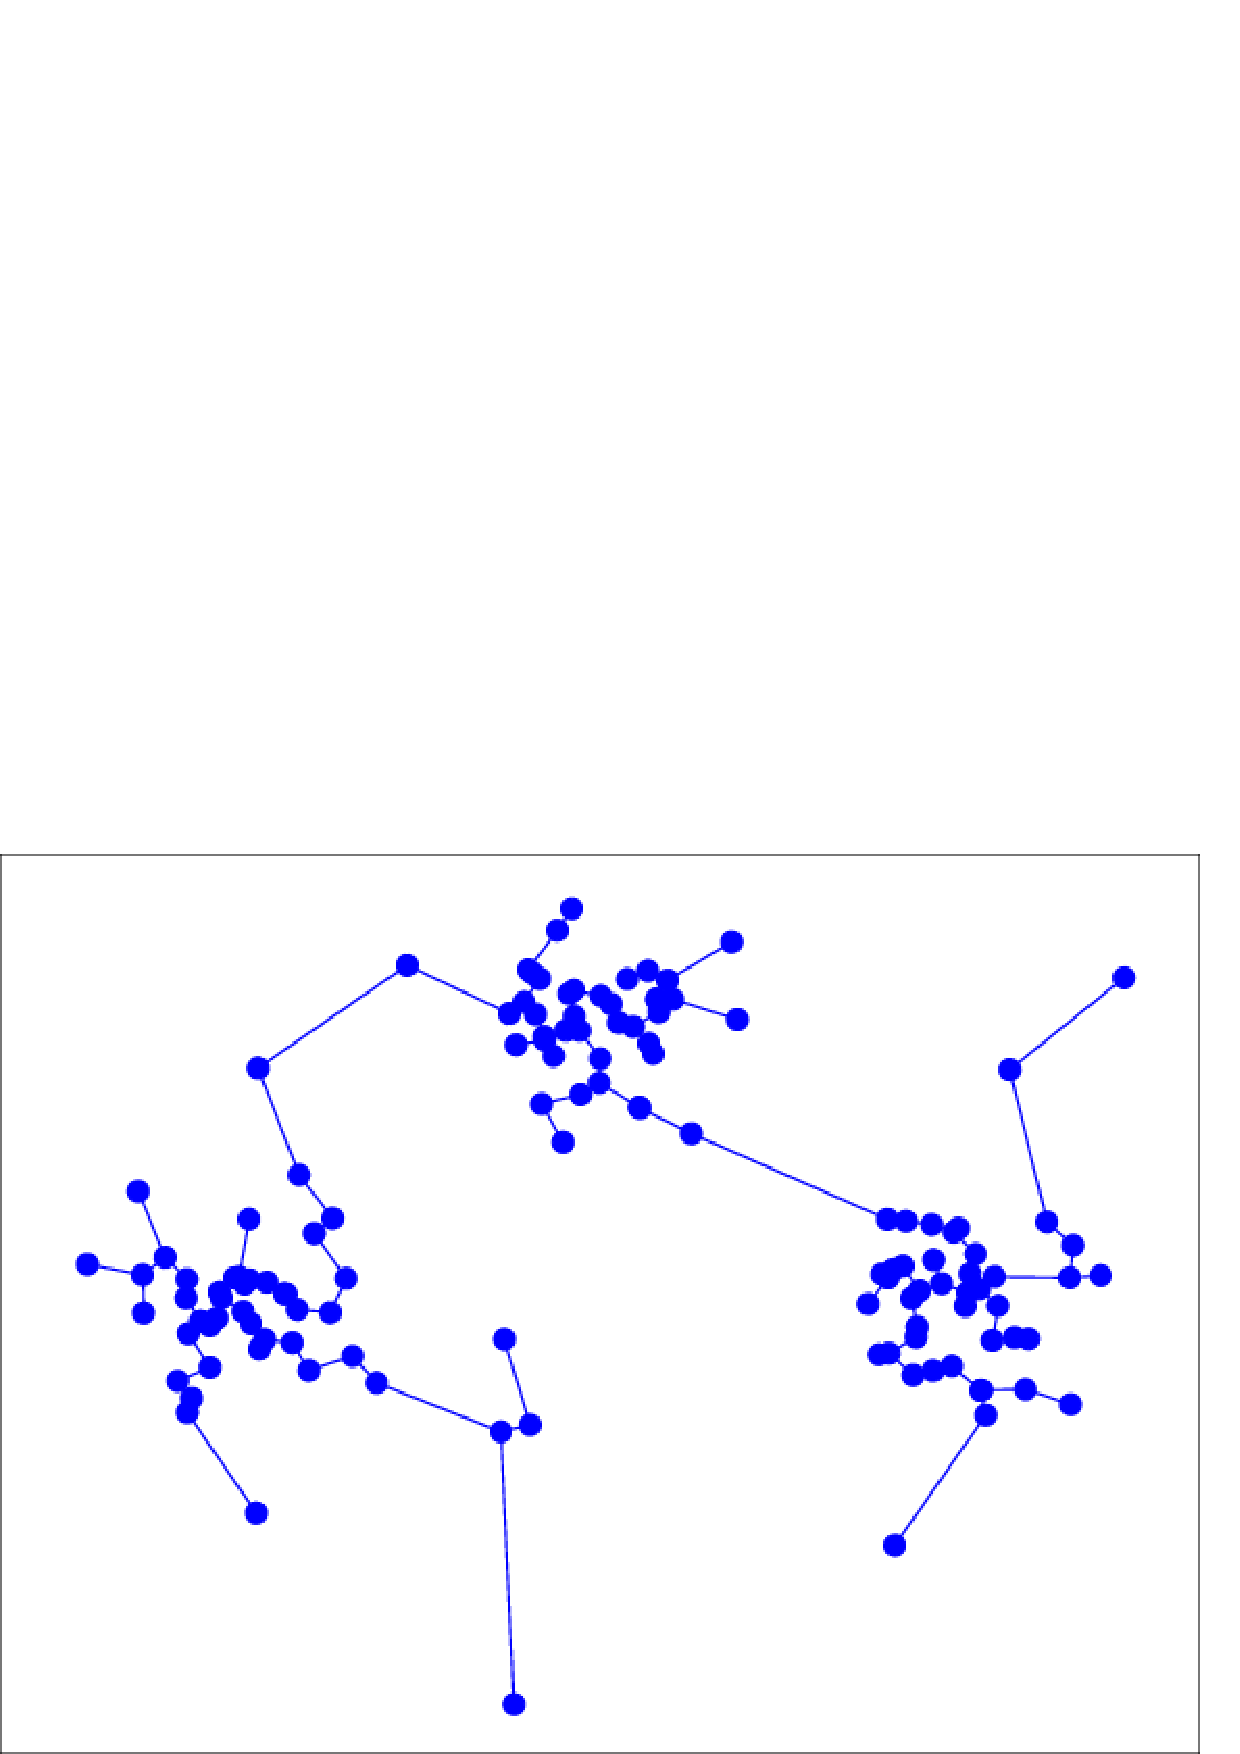
\includegraphics[width=.45\textwidth]{times_MNIST}
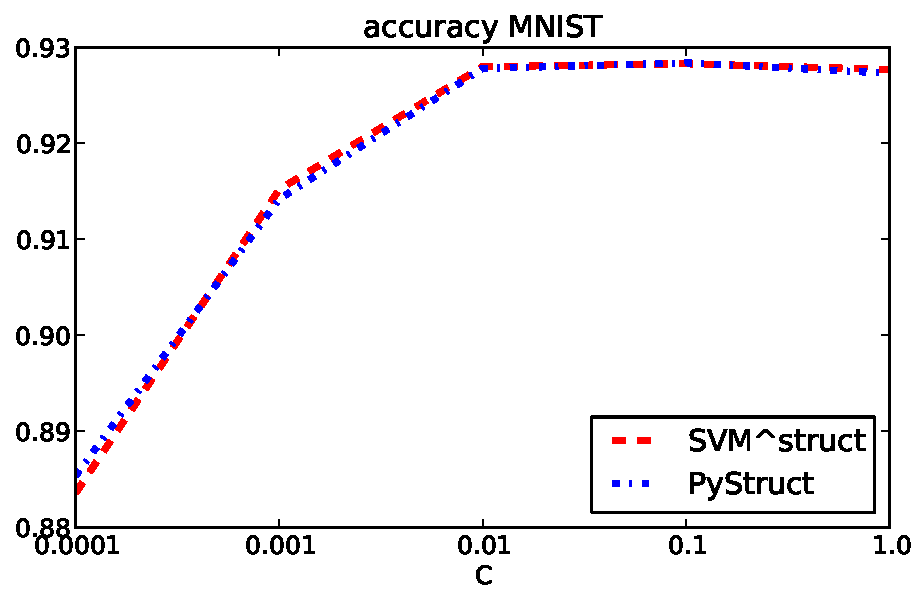
\includegraphics[width=.45\textwidth]{accs_MNIST}
\caption{Runtime comparison of \pystruct and \svmstruct for multi-class
    classification.
}
\label{fig:timings}
\end{figure}


\section{Summary}
%TODO summarize structured prediction
This chapter introduced \pystruct, a modular structured learning and prediction library in Python.
\pystruct is geared towards ease of use, while providing efficient implementations.
\pystruct integrates itself into the scientific Python eco-system, making it easy to use with
existing libraries and applications.
Currently, \pystruct focuses on max-margin and perceptron-based approaches. In the future,
we plan to integrate other paradigms, such as sampling-based learning~\citep{wick2011samplerank},
surrogate objectives (for example pseudo-likelihood), and approaches that allow for a better integration
of inference and learning~\citep{meshi2010learning}.
